% Parameters of the paper.
\documentclass[12pt,a4paper]{report}
\setlength\textwidth{160mm}
\setlength\textheight{247mm}
\setlength\oddsidemargin{0mm}
\setlength\evensidemargin{0mm}
\setlength\topmargin{0mm}
\setlength\headsep{0mm}
\setlength\headheight{0mm}
\let\openright=\clearpage

%\usepackage[czech]{babel}  % Czech
\usepackage{babel}          % English
\usepackage{lmodern}        %
\usepackage[T1]{fontenc}    % Change the font
\usepackage{textcomp}       %

\usepackage[utf8]{inputenc} % Coding.

%%% Další užitečné balíčky (jsou součástí běžných distribucí LaTeXu)
\usepackage{amsmath}        % rozšíření pro sazbu matematiky
\usepackage{amsfonts}       % matematické fonty
\usepackage{amsthm}         % sazba vět, definic apod.
\usepackage{bbding}         % balíček s~nejrůznějšími symboly
\usepackage{bm}             % tučné symboly (příkaz \bm)
\usepackage{graphicx}       % vkládání obrázků
\usepackage{fancyvrb}       % vylepšené prostředí pro strojové písmo
\usepackage{indentfirst}    % zavede odsazení 1. odstavce kapitoly
\usepackage{natbib}         % zajištuje možnost odkazovat na~literaturu
\usepackage[nottoc]{tocbibind} % zajistí přidání seznamu literatury,
                            % obrázků a tabulek do~obsahu
\usepackage{icomma}         % inteligetní čárka v~matematickém módu
\usepackage{dcolumn}        % lepší zarovnání sloupců v~tabulkách
\usepackage{booktabs}       % lepší vodorovné linky v~tabulkách
\usepackage{paralist}       % lepší enumerate a itemize
\usepackage{xcolor}         % barevná sazba
                            %
\usepackage{caption}        % Packages pro subfigures.
\usepackage{subcaption}     %
\usepackage{pdfpages}       % Vkladani pdfka.
\usepackage{hyperref}       % Odkazy.
\usepackage{tikz}           % Grafy a obrázky.
\usepackage{algpseudocode}  % Pseudokód
\usepackage{algorithm}
\usepackage{titling}
\usepackage{amssymb}

\usepackage{pgfplots}

%%% Tento soubor obsahuje definice různých užitečných maker a prostředí %%%
%%% Další makra připisujte sem, ať nepřekáží v ostatních souborech.     %%%

%%% Drobné úpravy stylu

% Tato makra přesvědčují mírně ošklivým trikem LaTeX, aby hlavičky kapitol
% sázel příčetněji a nevynechával nad nimi spoustu místa. Směle ignorujte.
\makeatletter
\def\@makechapterhead#1{
  {\parindent \z@ \raggedright \normalfont
   \Huge\bfseries \thechapter. #1
   \par\nobreak
   \vskip 20\p@
}}
\def\@makeschapterhead#1{
  {\parindent \z@ \raggedright \normalfont
   \Huge\bfseries #1
   \par\nobreak
   \vskip 20\p@
}}
\makeatother

% Toto makro definuje kapitolu, která není očíslovaná, ale je uvedena v obsahu.
\def\chapwithtoc#1{
\chapter*{#1}
\addcontentsline{toc}{chapter}{#1}
}

% Trochu volnější nastavení dělení slov, než je default.
\lefthyphenmin=2
\righthyphenmin=2

% Zapne černé "slimáky" na koncích řádků, které přetekly, abychom si
% jich lépe všimli.
\overfullrule=1mm

%%% Makra pro definice, věty, tvrzení, příklady, ... (vyžaduje baliček amsthm)

\theoremstyle{plain}
\newtheorem{veta}{Věta}
\newtheorem{lemma}[veta]{Lemma}
\newtheorem{tvrz}[veta]{Tvrzení}

\theoremstyle{plain}
\newtheorem{definice}{Definice}
\newtheorem*{pozor}{Pozorování}
\newtheorem*{cvic}{Cvičení}
\newtheorem*{fakt}{Fakt}

\theoremstyle{remark}
\newtheorem*{dusl}{Důsledek}
\newtheorem*{pozn}{Poznámka}
\newtheorem*{prikl}{Příklad}

\theoremstyle{plain}
\newtheorem{thm}{Theorem}
%\newtheorem{lemma}[thm]{Lemma}
\newtheorem{claim}[thm]{Claim}

\theoremstyle{plain}
\newtheorem{defn}{Definition}
\newtheorem*{observ}{Observation}
\newtheorem*{exerc}{Exercise}
\newtheorem*{fact}{Fact}

\theoremstyle{remark}
\newtheorem*{cor}{Corollary}
\newtheorem*{rem}{Remark}
\newtheorem*{example}{Example}


%%% Prostředí pro důkazy

\newenvironment{dukaz}{
  \par\medskip\noindent
  \textit{Důkaz}.
}{
\newline
\rightline{$\qedsymbol$}
}

\newenvironment{myproof}{
	\par\medskip\noindent
	\textit{Proof}.
}{
	\newline
	\rightline{$\qedsymbol$}
}


%%% Prostředí pro sazbu kódu, případně vstupu/výstupu počítačových
%%% programů. (Vyžaduje balíček fancyvrb -- fancy verbatim.)

\DefineVerbatimEnvironment{code}{Verbatim}{fontsize=\small, frame=single}

%%% Prostor reálných, resp. přirozených čísel
\newcommand{\R}{\mathbb{R}}
\newcommand{\N}{\mathbb{N}}
\newcommand{\Z}{\mathbb{Z}}

%%% Užitečné operátory pro statistiku a pravděpodobnost
\DeclareMathOperator{\pr}{\textsf{P}}
\DeclareMathOperator{\E}{\textsf{E}\,}
\DeclareMathOperator{\var}{\textrm{var}}
\DeclareMathOperator{\sd}{\textrm{sd}}

%%% Příkaz pro transpozici vektoru/matice
\newcommand{\T}[1]{#1^\top}

%%% Vychytávky pro matematiku
\newcommand{\goto}{\rightarrow}
\newcommand{\gotop}{\stackrel{P}{\longrightarrow}}
\newcommand{\maon}[1]{o(n^{#1})}
\newcommand{\abs}[1]{\left|{#1}\right|}
\newcommand{\dint}{\int_0^\tau\!\!\int_0^\tau}
\newcommand{\isqr}[1]{\frac{1}{\sqrt{#1}}}

%%% Vychytávky pro tabulky
\newcommand{\pulrad}[1]{\raisebox{1.5ex}[0pt]{#1}}
\newcommand{\mc}[1]{\multicolumn{1}{c}{#1}}


% set up \maketitle to accept a new item
\predate{\begin{center}\placetitlepicture\large}
	\postdate{\par\end{center}}

% commands for including the picture
\newcommand{\titlepicture}[2][]{%
	\renewcommand\placetitlepicture{%
		\includegraphics[#1]{#2}\par\medskip
	}%
}
\newcommand{\placetitlepicture}{} % initialization

 % Use global macros.

\title{Flows, paths and cuts}
\author{Tomáš Turek}
\titlepicture[width=5in]{res/flow.pdf}
%\date{}

%% Titulní strana a různé povinné informační strany
\begin{document}
	\maketitle
	\tableofcontents
	\chapter{Introduction}

Firstly we remind some basics from flows and cuts. 

\section{Network flow}

\textbf{Flow} is defined on a \textbf{network}. Network is on a oriented graph $G = (V,E)$ and it has two special vertices $s,t \in V$ called source and target. Also we have a capacity, which is a mapping $c : E \to \R_{0}^{+}$. Flow then is a mapping $f : E \to \R_{0}^{+}$ which has two properties.

\begin{enumerate}
	\item $\forall e \in E: f(e) \leq c(e)$
	\item Kirchoff's law: $\forall v \neq s, t \in V: \sum_{uv \in E} f(uv) - \sum_{vu \in E} f(vu) = 0$
\end{enumerate}

\section{Min $s,t$-cut}

Now we also remind ourselves another term which is an $s,t$-cut. Which is a $M \subset E$ such that no $s,t$-path exists in $G' = (V, E \setminus M)$.

These basic terms can be generalized to a \textbf{multi-commodity flow} problem and \textbf{multi-cut} problem.
	\chapter{Multi-commodity problem}

On a graph $G = (V,E)$ and $k$ tuples $(s_{1}, t_{1}), (s_{2}, t_{2}), \dots, (s_{k}, t_{k}) \ in V^{2}$ known as \textbf{commodities} we can also define a network and a flow. Same as before we have a capacity $c: E \to \R_{0}^{+}$. These commodities are shared on the same resources.

We may define $\mathcal{P}_{i}$ as all paths between $s_{i}$ and $t_{i}$. And also $\mathcal{P} := \bigcup_{i = 1}^{k} \mathcal{P}_{i}$.

For a single commodity flow problem we could define an \textit{linear program} (LP):

$$
\begin{array}{rl}
	& \max \sum_{p \in \mathcal{P}_{st}} f_{p} \\
	\forall e \in E & \sum_{p: e \in p \in \mathcal{P}_{st}} f_{p} \leq c(e) \\
	& f \geq 0
\end{array}
$$

From this we may define an linear program denoted as \textbf{LP1} for multi commodity problem.

$$
\begin{array}{rl}
	& \max \sum_{p \in \mathcal{P}} f_{p} = \sum_{i = 1}^{k} \sum_{p \in \mathcal{P}_{i}} f_{p} \\
	\forall e \in E & \sum_{j = 1}^{k} \sum_{p: e \in p \in \mathcal{P}_{j}} f_{p} \leq c(e) \\
	& f \geq 0
\end{array}
$$

Alternatively we could define it by a single variables for flows on each edge. For multi commodity problem we would have $k$ flows which adds up to one single flow. Thus we can see that the problem is in $P$ (polynomial).

\section{Multi cut problem}

As a cuts for single flow we may define somewhat similiar definition. Such that between every tuple of $s_{i}$ and $t_{i}$ there is no such path. We will also look at a linear program which will be denoted as \textbf{LP2}.

$$
\forall e : x_{e} =
\left\{
\begin{array}{rl}
	1 & e \text{ in cut} \\
	0 & \text{otherwise}	
\end{array}
\right.
$$

$$
\begin{array}{rl}
	\Phi := & \min \sum_{e \in E} x(e) c(e) \\
	\forall i \in [k] \forall p \in \mathcal{P}_{i} & \sum_{e \in p \in \mathcal{P}_{i}} x(e) \geq 1 \\
	\text{(ILP)} & x(e) \in \{0, 1\} \\
	\text{(LP)} & x(e) \geq 0
\end{array}
$$

First ILP is integer linear program which is generally NP hard. Thus we will look on the relaxation of LP program. We may observe that we don't need to specify that $x(e) \geq 1$.

Now we may see that indeed \textbf{LP1} and \textbf{LP2} are dual programs. Thus resulting in knowing that the maximum flow is the same as minimum fractional cut.

\section{Example}

Before we continue we will take a look at a simple example (\ref{example}). The graph is as follows. All capacities are equal to $1$.

\begin{figure}[!h]\centering
	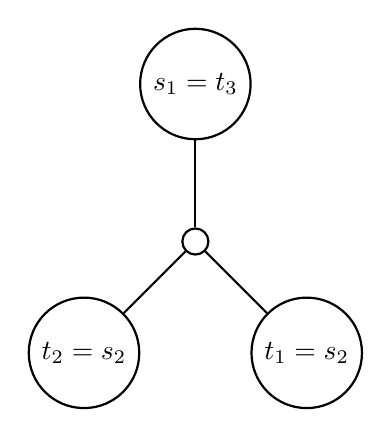
\begin{tikzpicture}[node distance={20mm}, thick, main/.style = {draw, circle}]
		\node[main] (1) {$s_{1} = t_{3}$};
		\node[main] (4) [below of=1] {};
		\node[main] (2) [below right of=4] {$t_{1} = s_{2}$};
		\node[main] (3) [below left of=4] {$t_{2} = s_{2}$};
		\draw (1) -- (4);
		\draw (4) -- (2);
		\draw (4) -- (3);
	\end{tikzpicture}
	\caption{Example graph.}
	\label{example}
\end{figure}

We may observe that the max flow is $|f| = \frac{3}{2}$ because we can put $\frac{1}{2}$ on every edge. Then multi-cut is $2$ since we need to remove always at least two edges. But minimum fractional multi-cut is only $\frac{3}{2}$ because we only have to "cut" half of each edge. Thus it is the exact same result as max flow.

\section{Preparation for algorithm}

We will show an algorithm which will give an approximate result of a multi-cut problem. We may look at it like we would cut off some parts of the graph which are close to the sources and continue.

Given $\bar{G} = (\bar{V}, \bar{E}), (s_{i}, t_{i}), k, c: E \to \R_{0}^{+}$ and solution $x$ of \textbf{LP2}. We define:

$$
B_{x}(s_{i}, r) := \{u \in \bar{V} | d_{x} (s_{i}, u) \leq r\}
$$

As a ball around $s_{i}$ with diameter w.r.t $x$. $d_{x} (s_{i}, u) :=$ the length of the shortest $s_{i}u$ path in $\bar{G}$ w.r.t. the edge length $x(e)$.

$$
\delta (B_{x}(s_{i}, r)) = \{\{u,v\} \in \bar{E} : |\{u,v\} \cap B_{x}(s_{i}, r)| = 1\}
$$

$$
V_{x}(s_{i}, r) = \frac{\Phi}{k} + \sum_{\{u,v\} \in \bar{E}, u,v \in B_{x}(s_{i},r)} c(e)x(e) + \sum_{\{u,v\} \in \delta(B_{x}(s_{i},r)): u \in B_{x}(s_{i},r)} c(e) (r - d_{x}(s_{i}, u))
$$

This we call a volume of a ball. We will denoted as a function of $r$ $f(r)$. The last sum is of all edges which are only partly inside the ball. Next we also define the following.

$$
C_{x}(s_{i}, r) = \sum_{\{u,v\} \in \delta(B_{x}(s_{i},r))} c(u,v)
$$

This will be denoted as a function $g(r)$. We may see some really nice properties these functions have. For instance $f(r)$ is a growing function which is increasing linearly and then it jumps to another point. On the other hand $g(r)$ is constant at some parts and then it jumps to a certain point, these jumps are for both function in the exact same spots. Next we can see that for some nice points it holds that $f'(r) = g(r)$.

\begin{lemma}
	For each $i \in [n]$ s.t. $s_{i}, t_{i} \in \bar{V}$ there exist $r \in (0, 1/2)$ s.t.
	
	$$
	\frac{C_{x}(s_{i}, r)}{V_{x}(s_{i},r)} \leq 2 \ln 2k.
	$$
\end{lemma}

\begin{myproof}
	By contradiction. For fixed $i$ $\forall r \in (0, 1/2)$, $\frac{f'(r)}{f(r)} > 2 \ln 2k$. We will have $r_{0} = 0 < r_{1} < r_{2} < \dots < r_{l-1} < 1/2 = r_{l}$ which are the values where $f(r)$ is not continuous (there are these "jumps"). First we consider $(r_{j}, r_{j+1})$ for some $j$.
	
	$$
	\frac{f'(r)}{f(r)} = \left( \ln f(r)\right)'
	$$
	
	So $\forall r \in (r_{j}, r_{j+1})$, $\left( \ln f(r)\right)' > 2 \ln 2k$. We will compute the integral over all of these values. We may see that the right side is just a constant so we get
	
	$$
	\int_{r_{j}}^{r_{j+1}} \left( \ln f(r)\right)' > (r_{j+1} - r_{j}) 2 \ln 2k.
	$$
	
	In $r_{j+1}$ there may be jump so we instead take the $\lim_{r \to r_{j+1}^{-}} f(r) = f^{-}(r_{j+1})$. Note that $f^{-}(r_{j+1}) \leq f(r_{j+1})$.
	
	$$
	\ln f(r_{j+1}) - \ln f(r_{j}) \geq \ln f^{-}(r_{j+1}) - \ln f(r_{j}) = \int_{r_{j}}^{r_{j+1}} \left( \ln f(r)\right)' > (r_{j+1} - r_{j}) 2 \ln 2k.
	$$
	
	Now we sum our inequality over all intervals $(r_{j}, r_{j+1}), j = 0, \dots, l$. We will only have the very ends because the rest will be once added and once removed.
	
	$$
	\sum_{j = 0}^{l-1} \left( \ln f(r_{j+1}) - \ln f(r_{j}) \right) > \sum_{j = 0}^{l-1} (r_{j+1} - r_{j}) 2 \ln 2k
	$$
	
	$$
	\ln f(r_{l}) - \ln f(r_{0}) > (r_{l} - r_{0}) 2 \ln 2k
	$$
	
	$$
	\ln f(1/2) - \ln (0) > \ln 2k
	$$
	
	$$
	\ln \frac{f(1/2)}{\frac{\Phi}{k}} > \ln 2k
	$$
	
	$$
	\frac{f(1/2)}{\frac{\Phi}{k}} > 2k
	$$
	
	$$
	f(1/2) > 2 \Phi
	$$
	
	As the volume of the entire pipe system is at most $2 \Phi$ it means that we have a contradiction.
\end{myproof}

Note that choosing $1/2$ is not necessary for the proof, but for the algorithm to work. Because if we choose $1/2$ it means that no $s_{j}, t_{j}$ will both be in a ball for the index $i$. That is because the length w.r.t $x$ of paths from $s_{j}$ to $t_{j}$ need to be at least $1$.

\section{Pipe cut algorithm}

\begin{algorithm}[!h]
	\caption{Pipe cut algorithm}
	\begin{algorithmic}[1]
		\Require $\bar{G} = (\bar{V}, \bar{E})$.
		\Ensure $F$ multi cut.
		\State $F \gets \emptyset$
		\For{$i = 1 \dots k$}
			\If{$s_{i}-t_{i}$ are still connected in $(\bar{V}, \bar{E} \setminus F)$}
				\State Choose $r \in (0, 1/2)$ by Lemma.
				\State $F \gets F \cup \delta(B_{x}(s_{i}, r))$
				\State Remove edges inside $B_{x}(s_{i}, r)$ and $\delta(B_{x}(s_{i}, r))$.
			\EndIf
		\EndFor \\
		\Return $F$
	\end{algorithmic}
\end{algorithm}



There are few things to talk about. To get $r$ we will check all "almost ends" of all intervals. The time complexity is polynomial since everything that is inside the code is polynomial. Correctness of the algorithm is easily observable since no pair $p_{i},t_{i}$ is inside some other ball and all balls will separate pairs $s_{j}, t_{j}$. Other thing to consider is what is the approximation ratio?

\begin{thm}
	Approximation ratio of the Pipe cut algorithm is $O(\log k)$.
\end{thm}

\begin{myproof}
	Lets define $C_{i}$ as the cost of the cut of the ball from iteration $i$ and $V_{i}$ as the volume of it. We know that $C_{i} \leq 2 \ln 2k \cdot V_{i}$.
	
	$$
	\sum_{i} C_{i} \leq 2 \ln 2k \sum_{i}V_{i} \leq 2 \ln 2k \cdot 2 \Phi = 4 \ln 2k \cdot \Phi = O (\log k) \Phi
	$$
\end{myproof}

For a single commodity we know that max flow $=$ min cut. Where $\leq$ is trivial and $\geq$ is a little harder. This is a case of \textbf{exact duality}. On the other hand we already shown that this doesn't hold for multi-commodity, but what if we can define \textbf{approximate duality}.

\begin{cor}
	Max flow $\leq$ min cut $\leq O(\log k)$ max flow. For multi-commodity.
\end{cor}

\begin{myproof}
	Because of the duality of LP1 and LP2 we know that max flow is the same as min fractional multi-cut. And because of the algorithm we know that the fractional multi-cut is in $O(\log k)$.
\end{myproof}

\section{How to solve LP}

There is still a problem with our LP which can have up to exponential many of constraints. But this can be solved fast by using \textbf{Ellipsoid algorithm} on $A x \leq b$. Only think it needs is an so called \textbf{ORACLE} which is that for given $\bar{x}$, check whether $A\bar{x} \leq b$ and if not return a violated constraint.

In our case \textbf{ORACLE} is for each $i$ find the shortest $s_{i}-t_{i}$ path w.r.t $\bar{x}$. This can be either $1$ and we are happy or $< 1$ then this constraint is violated.

\section{Is there any better approximation?}

We will show that indeed this approximation is the best we can get. Firstly we will define a new property of graphs.

A graph $G = (V,E)$ is an \textbf{$\alpha$-expander} if $\forall S \subseteq V, |S| \leq \frac{n}{2}, \delta(S) \leq \alpha |S|$.

We take as granted that it holds: $3$-regular $\alpha$-expanders exist for $\alpha > 0$. Now lets observe (\ref{3-regular})that at most $1 + 3 \cdot 2^{l-1}$ vertices are reachable by a path of length $\leq l$.

\begin{figure}[!h] \centering
	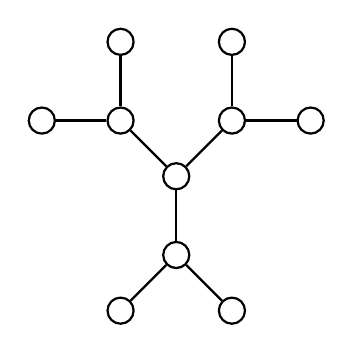
\begin{tikzpicture}[node distance={10mm}, thick, main/.style = {draw, circle}]
		\node[main] (1) {};
		\node[main] (2) [below of=1] {};
		\node[main] (3) [above right of=1] {};
		\node[main] (4) [above left of=1] {};
		\node[main] (5) [below left of=2] {};
		\node[main] (6) [below right of=2] {};
		\node[main] (7) [above of=3] {};
		\node[main] (8) [right of=3] {};
		\node[main] (9) [above of=4] {};
		\node[main] (10) [left of=4] {};
		\draw (1) -- (4);
		\draw (1) -- (2);
		\draw (1) -- (3);
		\draw (2) -- (5);
		\draw (2) -- (6);
		\draw (3) -- (7);
		\draw (3) -- (8);
		\draw (4) -- (9);
		\draw (4) -- (10);
	\end{tikzpicture}
	\caption{How to get the upper bound.}
	\label{3-regular}
\end{figure}

If we take $l = \log_{2} \frac{n-2}{6} + 1$ so with the upper bound we get $1 + 3\frac{n-2}{6} = 1 + \frac{n-2}{2} = \frac{n}{2}$. And also we define an instance of multi-commodity problem: $T = \{\{u,v\} | \delta(u,v) > l\}$. A unit of flow consumes $\geq l$ units of volume of the entire system. Thus $|E| = O(n)$. Therefore max flow $\leq O(\frac{n}{l}) = O(\frac{n}{\log n})$. But for min cut we take the optimum $F \subseteq E$. Every path in $G = (V, E \setminus F)$ is $\leq \frac{n}{2}$ so min cut os $\Theta(n)$. Thus it is indeed tight.
	\chapter{The Sparsest cut problem}

Same as before we have an undirected graph $G = (V,E)$ and $k$-pairs of sources and targets $(s_{1},t_{1}), (s_{2}, t_{2}), \dots, (s_{k}, t_{k}) \in V^{2}$. But we will introduce a new parameters $d_{1}, d_{2}, \dots, d_{k} \in \R^{+}$ called \textbf{demands}.

Firstly we will take a look at linear program for solving this problem for $k = 1$.

$$
\begin{aligned}
	\max f \\
	\sum_{p \in \mathcal{P}_{st}} x_{p} \geq f \cdot d_{1} \\
	\sum_{e \in \mathcal{P}_{st}} x_{p} \leq c(e) & \quad \forall e \in E\\
	x \geq 0
\end{aligned}
$$

Where $\mathcal{P}_{st}$ are all paths between $s$ and $t$. We may see that the optimum of the max flow is the same as this optimum just divided by $d_{1}$. We will denote $\mathcal{P}_{i} = \mathcal{P}_{s_{i}, t_{i}}$.

\section{Concurrent multicommodity flow}

Thus we are getting this LP for all $k$ commodities and $k$ demands.

$$
\begin{aligned}
	\max f \\
	\sum_{p \in \mathcal{P}_{i}} x_{p} \geq f \cdot d_{i} & \quad \forall i \in [k]\\
	\sum_{i = 0}^{k} \sum_{e \in \mathcal{P}_{i}} x_{p} \leq c(e) & \quad \forall e \in E\\
	x \geq 0
\end{aligned}
$$

We will take a look at the matrix of this LP and after that find a dual program. But firstly we modify $\sum_{p \in \mathcal{P}_{i}} x_{p} \geq f \cdot d_{i}$ to $f \cdot d_{i} - \sum_{p \in \mathcal{P}_{i}} x_{p} \leq 0$. Then the matrix is as follows:

$$
\begin{matrix}
	  & f     &    & \mathcal{P}_{1} &       &    & \mathcal{P}_{2} &       & \dots \\
	1 & d_{1} & -1 & -1              & \dots &  0 & \dots           & 0     & \dots \\
	2 & d_{2} & 0  &  0              & \dots & -1 & -1              & \dots & 0     \\
	\vdots  \\
	k & d_{k} & 0  &  0              & \dots & 0 & 0               &  0    & \dots \\
	e_{1} & 0     & 1  &  0              &       & 1 & 0               &  0    & \dots \\
	\vdots \\
	e_{|E|} & 0     & 0  &  1              &       & 1 & 0               &  1    & \dots \\
\end{matrix}
$$

Where for the first $k$ lines are $\leq 0$ and for edges it is $\leq c(e)$. We visualized the matrix and thus we can make the dual. We will have variables $x_{e}$ for edges and $y_{i}$ for $i \in [k]$. Thus the dual is:

$$
\begin{aligned}
	\min \sum_{e \in E} x_{e}c(e) \\
	\sum_{i = 0}^{k} y_{i}d_{i} \geq 1 \\
	\sum_{e \in p} x_{e} -y_{i} \geq 0 & \quad \forall i \in [k] \forall p \in \mathcal{P}_{i}\\
	x,y \geq 0
\end{aligned}
$$

\begin{defn}
	For $S \subseteq V$ we define $\delta(S) = \{\{u,v\} \in E : |\{u,v\} \cap S| = 1\}$ and then $I(S) = \{i \in [k] : |\{s_{i}, t_{i}\} \cap S| = 1\}$. Then the \textbf{sparsity} of $S$ is
	
	$$
	\rho(S) = \frac{\sum_{e \in \delta(S)}c(e)}{\sum_{i \in I(S)} d_{i}}
	$$
\end{defn}

\begin{example}
	We will have a simple example where all capacities are 1 and all demands are 1. So we have the graph \ref{example-sparse}. Note that there are 4 pairs of $s_i, t_i$ which can be seen by their demands.
	
	\begin{figure}[!h]\centering
		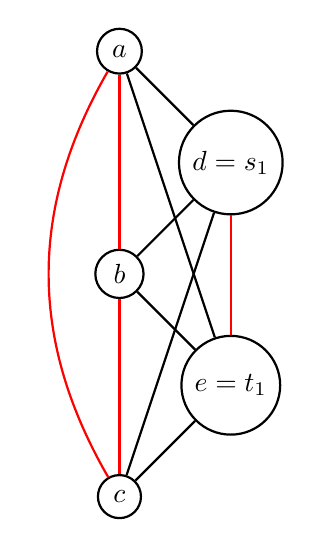
\begin{tikzpicture}[node distance={20mm}, thick, main/.style = {draw, circle}]
			\node[main] (1) {$a$};
			\node[main] (2) [below right of=1] {$d = s_{1}$};
			\node[main] (3) [below left of=2] {$b$};
			\node[main] (4) [below right of=3] {$e = t_{1}$};
			\node[main] (5) [below left of=4] {$c$};
			\draw (1) -- (2);
			\draw (1) -- (4);
			\draw (3) -- (2);
			\draw (3) -- (4);
			\draw (5) -- (2);
			\draw (5) -- (4);
			\draw [red] (1) -- (3);
			\draw [red] (5) -- (3);
			\draw [red] (2) -- (4);
			\path (1) edge [bend right, red] (5);
		\end{tikzpicture}
		\caption{Sparse cut example.}
		\label{example-sparse}
	\end{figure}
	
	The demands are the red edges. We may see that if we choose $S = \{c, e\}$ then $\sum_{e \in \delta(S)} c(e) = 3$ and $\sum_{i \in I(S)} d_{i} = 3$ therefore $\rho(S) = 1$.
	
	We may see that each pair $s_{i}$ $t_{i}$ consumes at least 2 units of a flow of the network for a single unit of the flow. Then we set $f$ as a max flow and see what we get. For example for paths $\mathcal{P}_{1} = \{(d,a,e) = p_{1}, (d,b,e) = p_{2}, (d,c,e) = p_{3}\}$. $x_{p_{1}} + x_{p_{2}} + x_{p_{3}} \geq f \cdot d_{1} = f$. Thus the total volume consumed by a flow with objective value $f$ is $\geq k 2 f = 8f$. Total volume of $G$ is 6. Therefore $f \leq \frac{6}{8} = \frac{3}{4}$.
	
	Maybe we can ask if there exist such a flow with this volume. We can obtain it by pushing $\frac{1}{4}$ from $d$ to $e$ on each path. And $\frac{3}{8}$ between all other pairs on all paths. All edges are not over their capacities and we get $\frac{3}{4}$ for all demands. Therefore we obtain following graph on picture \ref{max sparsest cut}. Hence there are 3 paths from $d$ to $e$ so in total it is $3/4$ and there two paths from $a$ to $b$ (and other pairs are same) therefore in total $6/8 = 3/4$.
	
	\begin{figure}[!h]\centering
		\begin{subfigure}{0.45\textwidth}\centering
			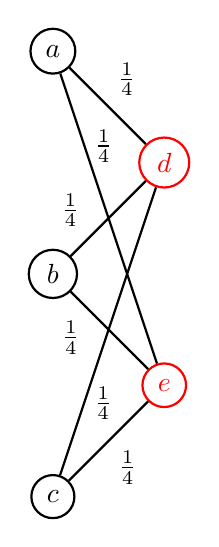
\begin{tikzpicture}[node distance={20mm}, thick, main/.style = {draw, circle}]
				\node[main] (1) {$a$};
				\node[main, color = red] (2) [below right of=1] {$d$};
				\node[main] (3) [below left of=2] {$b$};
				\node[main, color = red] (4) [below right of=3] {$e$};
				\node[main] (5) [below left of=4] {$c$};
				\draw (1) -- (2) node[midway, above right] {$\frac{1}{4}$};
				\draw (1) -- (4) node[near start, right] {$\frac{1}{4}$};
				\draw (3) -- (2) node[near start, above left] {$\frac{1}{4}$};
				\draw (3) -- (4) node[near start, below left] {$\frac{1}{4}$};
				\draw (5) -- (2) node[near start, right] {$\frac{1}{4}$};
				\draw (5) -- (4) node[midway, below right] {$\frac{1}{4}$};
			\end{tikzpicture}
			\caption{Paths from $d$ to $e$.}
		\end{subfigure}
		\begin{subfigure}{0.45\textwidth}\centering
			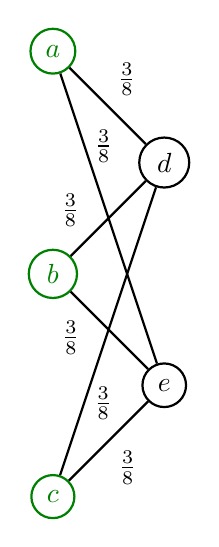
\begin{tikzpicture}[node distance={20mm}, thick, main/.style = {draw, circle}]
				\node[main, color = Green] (1) {$a$};
				\node[main] (2) [below right of=1] {$d$};
				\node[main, color = Green] (3) [below left of=2] {$b$};
				\node[main] (4) [below right of=3] {$e$};
				\node[main, color = Green] (5) [below left of=4] {$c$};
				\draw (1) -- (2) node[midway, above right] {$\frac{3}{8}$};
				\draw (1) -- (4) node[near start, right] {$\frac{3}{8}$};
				\draw (3) -- (2) node[near start, above left] {$\frac{3}{8}$};
				\draw (3) -- (4) node[near start, below left] {$\frac{3}{8}$};
				\draw (5) -- (2) node[near start, right] {$\frac{3}{8}$};
				\draw (5) -- (4) node[midway, below right] {$\frac{3}{8}$};
			\end{tikzpicture}
			\caption{Flows between the rest of the pairs.}
		\end{subfigure}
		\caption{Maximal sparsest flow $f$ in $G$.}
		\label{max sparsest cut}
	\end{figure}
\end{example}

\begin{defn}
	Now $F \subseteq E : I(F) = \{i \in [k] : s_{i}, t_{i} \text{ are in different components in } (V, E \setminus F)\}$. And \textbf{sparsity} of $F$ be
	
	$$
	\rho(F) = \frac{\sum_{e \in F}c(e)}{\sum_{i \in I(F)} d_{i}}
	$$
\end{defn}

\begin{lemma}
	$\min_{S \subseteq V} \rho(S) = \min_{F \subseteq E} \rho(E)$.
\end{lemma}

\begin{proof}
	The $\geq$ inequality can be easily seen if we set $F$ to be $\delta(S)$. Now we need to show the other inequality. For given $F \subseteq E$, let $s_{1}, \dots s_{l}$ be the components of connectivity of $(V, E \setminus F)$. For that we will proof that $\min_{i \in [l]} \rho(s_{i}) \leq \rho(F)$. This will bw shown by a contradiction. Assume $\forall i$:
	
	$$
	\begin{aligned}
		\frac{\sum_{e \in \delta(s_{i})}c(e)}{\sum_{j \in I(s_{i})} d_{j}} &> \frac{\sum_{e \in F}c(e)}{\sum_{j \in I(F)} d_{j}}\\
		\sum_{e \in \delta(s_{i})}c(e) &> \rho(F) \cdot \sum_{j \in I(s_{i})} d_{j}
	\end{aligned}
	$$
	
	Now we sum all $i$ inequalities.
	
	$$
	\sum_{i = 1}^{l} \sum_{e \in \delta(s_{i})}c(e) > \rho(F) \cdot \sum_{i = 1}^{l} \sum_{j \in I(s_{i})} d_{j}
	$$

	We can see that $\sum_{i = 1}^{l} \sum_{e \in \delta(s_{i})}c(e) = 2 \sum_{e \in F} c(e)$ because all edges are counted twice and similarly $\sum_{i = 1}^{l} \sum_{j \in I(s_{i})} d_{j} = 2 \sum_{j \in I(F)} d_{j}$. So we get:
	
	$$
	\sum_{e \in F} c(e) > \rho(F) \cdot \sum_{j \in I(F)} d_{j}
	$$
	
	Which is a contradiction. So for each $F$ we can find $s_{i}$ that satisfies the inequality.
\end{proof}

Now we can use this for integer program and then use relaxation. The program will look like this:

$$
\begin{aligned}
	\min \frac{\sum_{e \in E} c(e) x_{e}}{\sum_{i = 1}^{k}d_{i}y_{i}} \\
	\sum_{e \in p} x_{e} \geq y_{i} & \quad \forall i \in [k] \forall p \in \mathcal{P}_{i}\\
	\sum_{i = 1}^{k} d_{i}y_{i} \geq 1 \\
	x_{e} \in \{0,1\} &\quad \forall e \in E\\
	y_{i} \in \{0,1\} &\quad \forall i \in [k]
\end{aligned}
$$

At least one edge has to be removed from each path. Plus we assume that $d_{i} \geq 1$. Now we could just put $x_{e} \geq 0$ and $y_{i} \geq 0$. But the thing is that we don't have a linear function in the objective function. What if we have a vector $(x,y) \to (\alpha x, \alpha y)$ for $\alpha > 0$. You can see that the feasible solution don't change and also the objective is the same. So we could put $\alpha = \frac{1}{\sum_{i = 1}^{k} d_{i}y_{i}}$ and we know that the $\sum_{i = 1}^{k} d_{i}y_{i} = 1$. Thus the linear program will be:

$$
\begin{aligned}
	\min \sum_{e \in E} c(e) x_{e} \\
	\sum_{e \in p} x_{e} \geq y_{i} &\quad \forall i \in [k] \forall p \in \mathcal{P}_{i}\\
	\sum_{i = 1}^{k} d_{i}y_{i} = 1 \\
	x_{e} \geq 0 &\quad \forall e \in E\\
	 y_{i} \geq 0 &\quad \forall i \in [k]
\end{aligned}
$$

Before we continue we remind ourselves the Manhattan distance $||z||_{1} = \sum_{j=1}^{k} |z_{j}|$. This is indeed a metric, which means that it is non-negative, symmetric and triangular inequality holds.

\begin{lemma}
	Let $f$ be a mapping $f: V \to \R^{d}$ for some $d > 0$ and let
	
	$$
	\begin{array}{r r c l}
		\forall \{u,v\} \in E: & \hat{x}(\{u,v\}) & = & ||f(u) - f(v)||_{1} \\
		\forall i \in [k]: & \hat{y}(i) & = & ||f(s_{i}) - f(t_{i})||_{1} \\
		& \beta & = & \sum_{i = 1}^{k} d(i) \hat{y}(i).
	\end{array}
	$$
	
	Then $\left(\frac{\hat{x}}{\beta}, \frac{\hat{y}}{\beta}\right)$ is feasible solution. Also this is called \textbf{solution induced by $f$}. And we will denote $\left(\frac{\hat{x}}{\beta}, \frac{\hat{y}}{\beta}\right) = \left(x', y'\right)$.
\end{lemma}

\begin{proof}
	We need to show that all conditions of LP are satisfied. Easily the non-negativity still holds. Also
	
	$$
	\sum_{i=1}^{k} y'(i) d(i) = \sum_{i=1}^{k} \frac{\hat{y}(i)}{\beta}d(i) = 1
	$$
	
	where the last equality holds by the definition of $\beta$. Lastly we need to check that $\sum_{e \in E} x(e) \geq y(i)$ of our LP still holds. This can be easily proven by the fact that $||\cdot||_{1}$ is metric so in particular triangular inequality is satisfied and by induction on the length of the path we would prove it. Also keep in mind that scaling by $\beta$ doesn't change anything for the whole inequality since it is on both sides.
\end{proof}

\begin{lemma}[A]\label{A}
	Let $(x',y')$ be a solution induced by $f : V \to \R^{d}$. Then one can find in polynomial time cut $S \subseteq V$ of sparsity $\rho(S) \leq \sum_{e \in E} x'(e) c(e)$.
\end{lemma}

\begin{lemma}[B]\label{B}
	Given any feasible solution $(x,y)$ of LP, one can construct a mapping $f: V \to \R^{d}$ (by random algorithm with high probability) which induces a solution $(\bar{x}, \bar{y})$ s.t.
	
	$$
	\sum_{e \in E} c(e) \bar{x}(e) = O(\log k) \sum_{e \in E} c(e) x(e)
	$$
\end{lemma}

\begin{thm}
	There exist a randomized polynomial-time algorithm for the sparsest cut problem that is $O(\log k)$-approximation.
\end{thm}

\begin{proof}
	By Lemma B (\ref{B}) we generate $(\bar{x}, \bar{y})$ and then by Lemma A (\ref{A}) we construct the cut.
\end{proof}

\begin{proof}[Proof of Lemma A \ref{A}]
	Given $f: V \to \R^{d}$ let
	
	$$
	\begin{array}{l r c l}
		\forall u,v \in V & \mu (u,v) & = & ||f(u) - f(v)||_{1}
	\end{array}
	$$
	
	For $S \subseteq V$ we define $\forall u,v \in V$
	
	$$
	\mu_{S}(u,v) =
	\left\{
	\begin{array}{l l}
		1 & \text{iff } |\{u,v\} \cap S| = 1 \\
		0 & \text{otherwise}
	\end{array}
	\right.
	$$
	
	This will be called \textbf{cut mapping} and we can easily see that it is non-negative, symmetric and triangular inequality is satisfied thus it is metric. Before we continue we will use another lemma.
	
	\begin{lemma}[lemma]\label{lemma}
		$\forall S \subseteq V \ \exists \lambda_{S} \geq 0$ s.t. $\forall u,v \in V: \mu(u,v) = \sum_{S \subseteq V} \lambda_{S} \mu_{S}(u,v)$. Moreover $|\{S | \lambda_{S} > 0\}| \leq n \cdot d$.
	\end{lemma}
	
	\begin{proof}[Proof of lemma \ref{lemma}]
		Consider the contribution of the first coordinate to $\mu(u,v)$: order the vertices according to $f_{1}$ where $f = (f_{1}, f_{2}, \dots, f_{d})$, s.t. $f_{1}(v_{1}) \leq f_{1}(v_{2}) \leq \dots \leq f_{1}v_{n}$. Now let $S(l) = \{v_{1}, \dots, v_{l}\}$ for $l \in [n]$. Consider any two vertices $v_{i},v_{j}$ s.t. $i > j$.
		
		$$
		f_{1}(v_{i}) - f_{1}(v_{j}) = \sum_{l=j}^{i-1} (f_{1}(v_{l+1}) - f_{1}(v_{l})) = \sum_{l = 1}^{n-1} (f_{1}(v_{l+1}) - f_{1}(v_{l})) \mu_{S(l)} (v_{i}, v_{j}) 
		$$
		
		Where $(f_{1}(v_{l+1}) - f_{1}(v_{l})) = \lambda_{S(l)}$. This can be used to prove this for all dimensions $f_{2}, \dots, f_{d}$ thus it is true for $f$.
	\end{proof}
	
	\begin{observ}
		For any non-negative numbers $a_{1}, \dots, a_{n}$ and positive numbers $b_{1}, \dots, b_{n}$ holds:
		
		$$
		\frac{\sum_{i = 1}^{n} a_{i}}{\sum_{i = 1}^{n} b_{i}} \geq \min_{i \in [n]} \frac{a_{i}}{b_{i}}
		$$
	\end{observ}
	
	\begin{proof}[Proof of observation]
		By a contradiciton assume $\forall j:$
		
		$$
		\begin{aligned}
			\frac{\sum_{i = 1}^{n} a_{i}}{\sum_{i = 1}^{n} b_{i}} &< \frac{a_{j}}{b_{j}}\\
			b_{j} \frac{\sum_{i = 1}^{n} a_{i}}{\sum_{i = 1}^{n} b_{i}} &< a_{j}\\
			\sum_{j} b_{j} \frac{\sum_{i = 1}^{n} a_{i}}{\sum_{i = 1}^{n} b_{i}} &< \sum_{j} a_{j}
		\end{aligned}
		$$
		
		Where the last line is summing all the inequalities together. We get a contradiction. \textit{Note that geometricaly that can be represent as vectors and values of the $\tan$ function and it would state that there is a $\tan$ smaller of one of the vectors than the sum of them.}
	\end{proof}
	
	Now we continue to proof the Lemma A.
	
	$$
	\sum_{e \in E} c(e) x'(e) = \frac{\sum_{e \in E}c(e) x'(e))}{\sum_{i = 1}^{k}y'(i) d(i)}
	$$
	
	Which is just a division by $1$ from the conditions in LP. Then by lemma:
	
	$$
	\begin{aligned}
		& = \frac{\sum_{e \in E} c(e) \sum_{S \subseteq V} \lambda_{S} \mu_{S}(e)}{\sum_{i =1}^{k} d(i) \sum_{S \subseteq V} \lambda_{S} \mu_{S}(s_{i},t_{i})}\\
		&= \frac{\sum_{S \subseteq V} \lambda_{S} \sum_{e \in E} c(e) \mu_{S}(e)}{\sum_{S \subseteq V} \lambda_{S} \sum_{i =1}^{k} d(i)  \mu_{S}(s_{i},t_{i})}\\
		&\geq \min_{S \subseteq V} \rho(S)
	\end{aligned}
	$$
	
	The last part is due to the previous observation and the fact that $\sum_{e \in E} c(e) \mu_{S}(e) = a_{S}$ and $\sum_{i =1}^{k} d(i)  \mu_{S}(s_{i},t_{i}) = b_{S}$ taken means $\frac{a_{S}}{b_{S}} = \rho(S)$.
\end{proof}

Now we will be proving the Lemma A \ref{B}. For that we denote $T = \{s_{i} | i \in [k]\} \cap \{t_{i}| i \in [k]\}$ and without loss of generality assume that $|T| = 2^{\tau}$ (we can add arbitrary sources and targets that are essentially the same). Let us denote $d_{x} (u,v)$ the length of the $x$-shortest $u-v$ path. Where $x$ is the result of our LP. For $A \subseteq V: d_{x}(A,u) = \min_{v \in A} d_{x}(v,u)$.

Also we put $L = q \log (k)$ where $q$ is some constant to be decided later on and $k$ is for number of commodities. Also $d = L \cdot \tau = O (\log^{2}(k))$. For $t = 1, \dots, \tau$ and $l = 1, \dots, L$: let $A_{tl}$ be a set that is constructed by $2^{\tau - t}$-times selecting uniformely at random $v \in V$.

\begin{defn}
	$\forall v \in V: f_{tl}(v) = d_{x}(v, A_{tl})$.
\end{defn}

\textit{Note that both $A_{tl}$ and $f_{tl}$ are not dependent on $l$. One can say that $l$ is for repeating the selection.}

\begin{lemma}
	$\forall \{u,v\} \in E : || f(u) - f(v)||_{1} \leq d \cdot x(u,v)$.
\end{lemma}

\begin{proof}
	We proceed by the definition and some algebra.
	
	$$
	|| f(u) - f(v)||_{1} = \sum_{t = 1}^{\tau} \sum_{l = 1}^{L} |f_{tl}(u) - f_{tl}(v)| = \sum_{t = 1}^{\tau} \sum_{l = 1}^{L} |d_{x}(u, A_{tl}) - d_{x}(v, A_{tl})|
	$$
	
	Now lets take a look at these inequalities which follows from the triangle inequalities.
	
	$$
	\begin{array}{r c l}
		d_{x}(u, A_{tl}) & \leq & x(u,v) + d_{x}(v, A_{tl}) \\
		d_{x}(v, A_{tl}) & \leq & x(u,v) + d_{x}(u, A_{tl}) \\
		& \Downarrow & \\
		d_{x}(u, A_{tl}) - d_{x}(v,A_{tl}) & \leq & x(u,v) \\
		d_{x}(v, A_{tl}) - d_{x}(u,A_{tl}) & \leq & x(v,u)
	\end{array}
	$$
	
	Which leads to $|d_{x}(u,A_{tl}) - d_{x}(v, A_{tl})| \leq x(u,v)$ and thus getting the last inequality:
	
	$$
	\sum_{t = 1}^{\tau} \sum_{l = 1}^{L} |d_{x}(u, A_{tl}) - d_{x}(v, A_{tl})| \leq \tau \cdot L \cdot x(u,v) = d \cdot x(u,v)
	$$
\end{proof}

\begin{lemma}
	With probability $\geq 1/2$: $\forall i \in [k]$ holds that
	
	$$
	||f(s_{i}) - f(t_{i})||_{1} \geq \frac{L}{88} y_{i}.
	$$
\end{lemma}

Before proving this lemma we will take a look, how useful it is. $\beta = \sum_{i = 1}^{k} d(i) \cdot ||f(s_{i}) - f(t_{i})||_{1} = \Omega(\log k) \cdot \sum_{i = 1}^{k} d(i) y_{i} = \Omega(\log k)$ where $y_{i}$ is from our LP and thus $\sum_{i = 1}^{k} d(i) y_{i}$ is equal to 1. The second equality is from the lemma before. And now from the lemma even before that we get $\leq \sum_{e \in E} c(e) \cdot d \cdot x(e) = d \sum_{e \in E} c(e) x(e)$ which is the objective function result of our LP. Thus $= O(\log^{2}(k)) \sum_{e \in E} x(e) c(e)$. But that is scaled by $\beta$ thus the objective value of the solution induced by $f$ is $\leq O(\frac{\log^{2}(k)}{\log(k)} \sum_{e \in E} c(e) x(e) = O(\log k) \sum_{e \in E} x(e) c(e)$ and so we have $O(\log k)$-approximation. So this proves the Lemma B \ref{B}.

\begin{proof}
	To prove the lemma we will prove a simple version that for fixed $i \in [k]$ with probability $\geq 1 - 1/2k$ it holds that
	
	$$
	||f(s_{i}) - f(t_{i})||_{1} \geq \frac{L}{88} y_{i}.
	$$
	
	We can easily see that for doing this for all $i \in [k]$ the lemma will follow. To prove this we will define few more things.
	
	$$
	\begin{aligned}
		\forall v \in \{s_{i}, t_{i}\}: &\ B_{x}(v, r) = \{w \in T | d_{x}(v,w) \leq r\}\\
		\forall v \in \{s_{i}, t_{i}\}: &\ B_{x}^{\circ}(v, r) = \{w \in T | d_{x}(v,w) < r\}
	\end{aligned}
	$$
	
	Now we will look at this sequence of radii. $r_{0} = 0$,
	
	$$
	r_{t} = \min \{r > 0 : |B_{x}(s_{i},r)| \geq 2^{t} \land |B_{x}(t_{i},r)| \geq 2^{t}\}
	$$
	
	$$
	\hat{t} = \min \left\{t | r_{t} \geq \frac{y(i)}{4}\right\}
	$$
	
	and also redefine $r_{\hat{t}} = \frac{y(i)}{4}$. This is define with respect to LP. And also it means that $B_{x}(s_{i}, r_{\hat{t}}) \cap B_{x}(t_{i}, r_{\hat{t}}) = \emptyset$.
	
	Now we observe that for $A_{tl} \subseteq V:$ $A_{tl} \cap B_{x}^{\circ}(s_{i}, r_{t}) = \emptyset \Leftrightarrow d_{x}(s_{i}, A_{tl}) \geq r_{t}$. And also $A_{tl} \cap B_{x}(t_{i}, r_{t - 1}) \neq \emptyset \Leftrightarrow d_{x}(t_{i}, A_{tl}) \leq r_{t - 1}$. Let $E_{tl}$ be the event such that $A \cap B = \emptyset$ and $A \cap G \neq \emptyset$ where $B = B_{x}^{\circ}(s_{i}, r_{t})$ and $G = B_{x}(t_{i}, r_{t - 1})$.
	
	We may observe that if $E_{tl}$ happens then $|f_{tl}(s_{i}) - f_{tl}(t_{i})| = |d_{x}(s_{i}, A_{tl}) - d_{x}(t_{i}, A_{tl})| \geq r_{t} - r_{t -1}$. We will look at the  probability of happening this.
	
	$$
	\begin{aligned}
		\Pr[E_{tl}] & = \Pr[A_{tl} \cap G \neq \emptyset | A_{tl} \cap B = \emptyset] \Pr[A_{tl} \cap B = \emptyset] \\
		            & \geq \Pr[A_{tl} \cap G \neq \emptyset] \Pr[A_{tl} \cap B = \emptyset]
	\end{aligned}
	$$
	
	Let us assume wlog $s_{i}$ defines $r_{t}$.
	
	$$
	\Pr[A_{tl} \cap B = \emptyset] = \left( 1 - \frac{|B|}{|V|} \right) ^{2^{\tau - t}} \geq \left( 1 - \frac{2^{t}}{2^{\tau}} \right) ^{\frac{2^{\tau}}{2^{t}}} \geq \frac{1}{e} \geq \frac{1}{4}
	$$
	
	$$
	\Pr[A_{tl} \cap G \neq \emptyset] = (1 - \Pr[A_{tl} \cap G = \emptyset]) = 1 - \left( 1 - \frac{|G|}{|V|} \right)^{2^{\tau - t}} \geq
	$$
	
	$$
	\geq 1 - \left( 1 - \frac{2^{t -1}}{2^{\tau}} \right)^{\frac{2^{\tau}}{2^{t-1}} \frac{1}{2}} \geq 1 - \left( \frac{1}{e} \right)^{\frac{1}{2}} \geq \frac{4}{11}
	$$
	
	Thus the $\Pr[E_{tl}] \geq \frac{1}{11}$. Now we fix $t = \{1, \dots, \tau\}$ and define:
	
	$$
	X_{tl} = \left\{
	\begin{array}{l l}
		1 & \text{ iff } E_{tl} \text{ occurs} \\
		0 & \text{otherwise}
	\end{array}
	\right.
	$$
	
	For $l = 1, \dots, L$ let $\mu = \E \left[ \sum_{l = 1}^{L} X_{tl} \right]$. We may observe that $\mu \geq \frac{L}{11}$ by linearity of $\E$. We now may use the Chernoff bound.
	
	$$
	\Pr \left[ \sum_{l = 1}^{L} X_{tl} \leq \frac{\mu}{2} \right] \leq e^{\frac{-\mu}{8}} \leq e^{\frac{-q \log k}{88}} \leq e^{-\log 2k - \log\log2k} = \frac{1}{2k \log 2k}
	$$
	
	Where there is hidden analysis to proper choice of $q$. If $\sum_{l = 1}^{L} X_{tl} \geq \frac{\mu}{2}$ then
	
	$$
	\sum_{l = 1}^{L} |f_{tl}(s_{i}) - f_{tl}(t_{i})| \geq \sum_{l = 1}^{L} X_{tl} (r_{t} - r_{t-1}) \geq \frac{L}{22} (r_{t} - r_{t-1})
	$$
	
	Therefore with probability $\geq 1 - \frac{\tau}{2k \log 2k} \geq 1 - \frac{1}{2k}$ $\forall t \in [\hat{t}]$ the previous statement holds. Thus
	
	$$
	||f(s_{i}) - f(t_{i})||_{1} \geq \frac{L}{88} y_{i} = \frac{L}{88} 4 \sum_{t = 1}^{\tau} (y_{t} - y_{t-1})
	$$
\end{proof}

\section{Metric spaces}

Some of basic definitions are for metric spaces which reader may already know, but we will remind it once again.

\begin{defn}
	Metric space $(M,d)$ when $d : M \times M \to \mathbb{R}^{+}$ and
	
	\begin{enumerate}[(i)]
		\item $\forall x,y \in M: d(x,y) \geq 0$ and $d(x,y) = 0 \Leftrightarrow x = y$,
		\item $\forall x,y \in M : d(x,y) = d(y,x)$,
		\item $\forall x,y,z \in M: d(x,z) \leq d(x,y) + d(y,z)$.
	\end{enumerate}
\end{defn}

We may already know some examples. One is for $G = (V,E)$ and for $x : E \to \mathbb{R}^{+}$ the metric is $d(z,y) = \min_{z-y \text{ paths}} \sum_{e \in P} x(e)$. This means that $(V,d)$ is a metric system.

\begin{defn}
	Let $(X,d)$ and $(Y,\bar{y})$ be metric spaces. An injective function $f : X \to Y$ is $D$-embedding for some $D \geq 1$, if $\exists r > 0$ such that $\forall x,y \in X$ the following holds
	
	$$
	r \cdot d(x,y) \leq \bar{d}(f(x), f(y)) \leq D \cdot r \cdot d(x,y).
	$$
\end{defn}

\begin{defn}
	The $\inf$ of $D$ values satisfying the above property is called \textbf{distortion} of $f$.
\end{defn}

\begin{thm}[Bourgain, 1985]
	Every $n$-point metric space $(V,d)$ can be embedded in $(\mathbb{R}^{p}, l_{1})$ with distortion $O(\log n)$ with $p = O(\log ^{2} n)$. Where $l_{1} = ||x||_{1} = \sum_{i}x_{i}$.
\end{thm}

We remind ourselves what we did. We constructed $f : V \to \mathbb{R}^{+}$ and $p = O(\log^{2} k)$ such that

\begin{enumerate}[(i)]
	\item $\forall u,v \in V : ||f(u) - f(v)||_{1} \leq p \cdot d_{x}(u,v)$,
	\item $\forall i \in [k] : ||f(s_{i}) - f(t_{i})||_{1} \geq \Omega(\log k) d_{x}(s_{i}, t_{i})$.
\end{enumerate}

So if we take $T = V$, think about all pair of vertices as commodities. Everything in the proof still works. So we technically proved this theorem before.

Now the question one can ask is: \textit{Is the analysis tight?} For the answer we may recall that in 3-regular graphs, there are $\Omega (n^{2})$ pairs of vertices at distance $\Omega (\log k)$. That was for the multi-commodity system. Lets consider 3-regular $\beta$-expanders (i.e. $\delta (S) \geq \beta|S|, \forall S \subseteq V, |S| \leq |V|/2$).

With that consider the instance: Commodity for each pair of vertices and set all $d = 1$. This will lead to

$$
\min_{S \subseteq V} \frac{E(S, V \setminus S)}{I(S)} \geq \min_{S \subseteq V} \frac{\beta |S|}{|S| |V \setminus S|} \geq \frac{\beta}{|V|} = \Omega(1/n)
$$

then the max concurrent flow is at most the available capacity $O(n)$ divided by what unit of flow consumes. Thus get

$$
\frac{O(n)}{\Omega (n^{2} \log n)} = O\left( \frac{1}{n \log n} \right)
$$

which means that it is tight. Alternatively integrality gap of our LP is $\Omega(\log n)$. Also it implies that the asymptotic optimality of the theorem is tight. Otherwise if there was better version we could use that for better approximation of our LP which is a contradiction. Also there exists $O(\sqrt{\log n})$-approximation for sparsest cut using positive semidefinite programming.

\begin{cor}
	Max flow $\leq$ min cut $\leq O(\log k)$ max flow. For sparsest cut problem.
\end{cor}

\section{Applications}

\begin{defn}
	Cut $(S, V \setminus S)$ is $b$-balanced (for some $b \leq 1/2$) if
	
	$$
	b n \leq |S| \leq (1-b)n
	$$
	
	where $G = (V,E)$ and $|V| = n$.
\end{defn}

$1/2$-balanced is called \textbf{bisection}. Also there is a problem for finding a $b$-balanced cut minimizing the number of edge between $E(S, V \setminus S)$ (\textit{cost of cut}). This problem is generally NP-hard.

\begin{thm}
	If there is a $b$-balanced cut $T$ in $G = (V,E)$, then for any $b' < \min\{1/3, b\}$ one can find in polynomial time $b'$-balanced cut of cost $O \left(\frac{E(T, V \setminus T) \log n}{b-b'}\right)$.
\end{thm}

\begin{proof}
	First we define the algorithm.
	
	\begin{algorithm}
		\caption{Find $b'$-balanced cut.}
		\begin{algorithmic}[1]
			\Require Graph $G$.
			\Ensure $b'$-balanced cut.
			\State $i := 0$, $G_{i} = G$, $S = \emptyset$
			\While{$|V(G_{i})| > (1-b')|V| $}
			\State find an approximation of the sparsest cut in $G_{i}$ and denote it as $S_{i} \subseteq V(G_{i})$
			\State let $G_{i+1} = G_{i}[V(G_{i}) \setminus S_{i}]$, $S = S \cup S_{i}$, $i = i+1$
			\EndWhile
			\Return S
		\end{algorithmic}
	\end{algorithm}
	
	where in the sparsest cut problem is on the network where all vertices are terminals and demands are $1$.
	
	Correctness of the algorithm: Before the last iteration it is true that $|S| < b'n$. In the last iteration at most $|V(G_{i})| / 2$ are added to $S$. Therefore at the end
	
	$$
	\leq |S| + \frac{n - |S|}{2} = \frac{n + |S|}{2} < \frac{(1+ b')n}{2} \leq (1- b')n
	$$
	
	Where the last inequality is due the value $b' \leq 1/3$ and the fact that $1+b' \leq 2-2b'$. Also because it ended $|S| \geq b'n$ so it is indeed a $b'$-balanced cut.
	
	Approximation of the cost:	Consider an optimal $b$-balanced cut $(T, V \setminus T)$. In each iteration $|T \setminus S| \geq (b - b') n$. What is the sparsity of the cut $T \setminus S$? Lets denote $\text{opt} = E(T, V \setminus V)$. The sparsity is
	
	$$
	\leq \frac{\text{opt}}{b - b')n(1-b)n} \leq \frac{2 \text{opt}}{(b-b')n^{2}}
	$$
	
	so the sparsity of the $O(\log n)$-approximation $S_{i}$ found by the algorithm is
	
	$$
	\frac{E(S_{i}, V_{i} \setminus S_{i})}{|S_{i}| |V_{i} \setminus S_{i}|} \leq O(\log n) \frac{\text{opt}}{(b-b')n^{2}}
	$$
	
	which means that $E(S_{i}, V_{i} \setminus S_{i}) \leq O(\log n) \frac{\text{opt}}{(b-b')n^{2}} |S_{i}|$. Now we sum it up.
	
	$$
	E(S, V \setminus S) \leq \sum_{i} E(s_{i}, V_{i} \setminus S_{i}) \leq O(\log n) \frac{\text{opt}}{(b-b')n^{2}} \sum_{i} |S_{i}| = O(\log n) \frac{\text{opt}}{b - b'}
	$$
\end{proof}

\section{Minimum cut linear arrangement}

Given $G = (V,E)$, find ordering $v_1, \dots, v_n$ of the vertices such that

$$
\max_{i \subset [n]} E(\{v_{1}, \dots, v_{i}\}, \{v_{i}, \dots, v_{n}\}) \text{ is minimized.}
$$

\begin{observ}
	$OPT \geq \min$ bijection of $G = : \mathcal{B}$.
\end{observ}

\begin{proof}
	For any ordering $E(\{v_{1}, \dots, v_{n/2}\} \{v_{n/2 +1}, \dots, v_{n}\}) \geq B$.
\end{proof}

\begin{algorithm}
	\caption{Find minimum cut linear arrangement}
	\begin{algorithmic}[1]
		\Require{Graph $G$}
		\Ensure{Minimum cut linear arrangement}
		\State Find a $1/3$-balanced cut of $G$ and denote it as $(L,R)$ by the previous algorithm.
		\State Solve the problem recursively for $L,R$.
	\end{algorithmic}
\end{algorithm}

\begin{observ}
	The depth of recursion is $O(\log n)$.
\end{observ}

\begin{observ}
	$E(L,R) \leq O (\log n) \cdot B$.
\end{observ}

And now we would like to get similiar bound for all the levels of recursion. For that consider $G_{i}$. Lets denote $B_{i}$ the bijection of $G_{i}$ and $OPT_{i}$ the optimum solution for $G_{i}$. Then $B_{i} \leq OPT_{i} \leq OPT$, therefore in our solution

$$
\forall i \in [n], E(\{v_{1}, \dots, v_{i}\} \{v_{i+1}, \dots, v_{n}\}) \leq O(\log n) \cdot O(\log n) \cdot OPT
$$

because the first $O$ is for number of recursion calls and the second $O$ is approximation of the size of each balanced cut. Altogether it is equal to $O(\log^2 n) OPT$.

\begin{thm}
	The approximation ratio of the algorithm is $O(\log^2 n)$.
\end{thm}

\begin{defn}
	Crossing number of the graph is the number of intersections of edges (the minimum). For planar graphs it is 0 and for not planar it is $\geq 1$.
\end{defn}

This can be also solved by the algorithm above.
	\chapter{Max cut}

We have been talking about minimal cuts the whole time. Now we will consider somewhat opposite problem. That is for given graph $G = (V,E)$ we want to find $S \subseteq V$ such that $E(S, V \setminus S)$ is maximized.

For this problem we may introduce a \textbf{randomized algorithm} which is simple. For every vertex choose if it is in $S$ or in $V \setminus S$ with probability $1/2$. Then $\E [|E(S, V \setminus S)|] = \frac{|E|}{2} \geq \frac{OPT}{2}$ because the probability of edge being in the cut is exactly one half, since there are four options where $u$ and $v$ may land, but in two scenarios they are in the same part and in the rest they are on the opposite sites.

Now we would like to talk about $0,878\dots$-approximation. Firstly we will label our vertices. WLOG: $V = \{1, 2, \dots, n\}$. Set $\forall i \in V: y_{i}^2 =1$. Now think about an edge $ij$. How can we express with this representation of the graph that $ij$ is in the cut? Think about

$$
y_{i} \cdot y_{j} = \left\{
\begin{array}{r l}
	1 & \text{on the same side} \\
	-1 & \text{on different sides}
\end{array}
\right.
$$

and from this we would make

$$
\frac{1 - y_{i}\cdot y_{j}}{2} = \left\{
\begin{array}{r l}
	0 & \text{on the same side} \\
	1 & \text{on different sides}
\end{array}
\right..
$$

So with this we can introduce a maximalization problem:

$$
\max \frac{1}{2} \sum_{\{i,j\} \in E} (1 - y_i y_j)
$$

Altogether we can define a \textbf{quadratic formulation} for max-cut problem. Every part was already mentioned, but just to gather it on one place.

$$
\begin{aligned}
	\forall i \in V: y_{i}^2 = 1 \\
	\max \frac{1}{2} \sum_{\{i,j\} \in E} (1 - y_i y_j) \\
	y_{i} \in \R
\end{aligned}
$$

We may see that this program is not very good for solving. This means we will relax it to a \textbf{vector program} and we will denote it as VP for future usage.

$$
\begin{aligned}
	\max \frac{1}{2} \sum_{\{i,j\} \in E} (1 - y_i^T y_j) \\
	y_i^T y_i = 1 \\ 
	\forall i : y_{i} \in \R
\end{aligned}
$$

The intuition behind it is that we start with 1 dimensional ball (which are line segments $[-1,1]$) and then we will continue to higher dimensions. In the VP we use vectors instead of usual numbers. We will continue with changing the program. Now it will be to semi-positive programming or SPD for short. This formulation is as follows.

$$
\begin{aligned}
	\max \frac{1}{2} \sum_{\{i,j\} \in E} (1 - Y_{ij}) \\
	\forall i : Y_{ii} = 1 \\
	Y \text{ is positive semi-definite}
\end{aligned}
$$

When it is written in this form it can be solved in polynomial time. Just for a reminder we introduce a definition of PSD.

\begin{defn}
	We say that a symmetric matrix $A \in \R^{n \times n}$ is positive semi-definite if $\forall x : x^T A x \geq 0$.
\end{defn}

\begin{observ}
	$A$ is positive semi-definite $\Leftrightarrow \exists$ matrix $U \in \R^{n \times n}$ s.t. $A = U^T U$. 
\end{observ}

\begin{observ}
	VP = PSD
\end{observ}

\begin{proof}
	This is from the above observation because we can put the semi-positive matrix $Y$ to a multiplication of two matrices which will look like this:
	
	$$
	\begin{pmatrix}
		\dots & y_1 & \dots \\
		& \vdots & \\
		\dots & y_n & \dots \\
	\end{pmatrix}
	\begin{pmatrix}
		\vdots &  & \vdots \\
		y_1 & \dots & y_n\\
		\vdots &  & \vdots \\
	\end{pmatrix}
	$$
\end{proof}

\begin{algorithm}
	\caption{Algorithm for max cut}
	\begin{algorithmic}[1]
		\Require{Graph $G$}
		\Ensure{$S$ max cut of $G$.}
		\State Solve SDP.
		\State Interpret it as a solution of the VP $\to v_{1}, \dots, v_{n} \in \R^n$.
		\State Sample uniformly at random $r \in \{x \in \R^n : x^2 = 1\}$
		\State \Return $S = \{i \in V : v_{i}^T r \geq 0\}$.
	\end{algorithmic}
\end{algorithm}

We know that both $v_{i}$ and $r$ are unit vectors. So $\cos \alpha = v_{i}^T \cdot r$. Where the $\cos$ function can be seen on a picture \ref{cos} to visualize how it looks.

\begin{figure}[!ht]\centering
	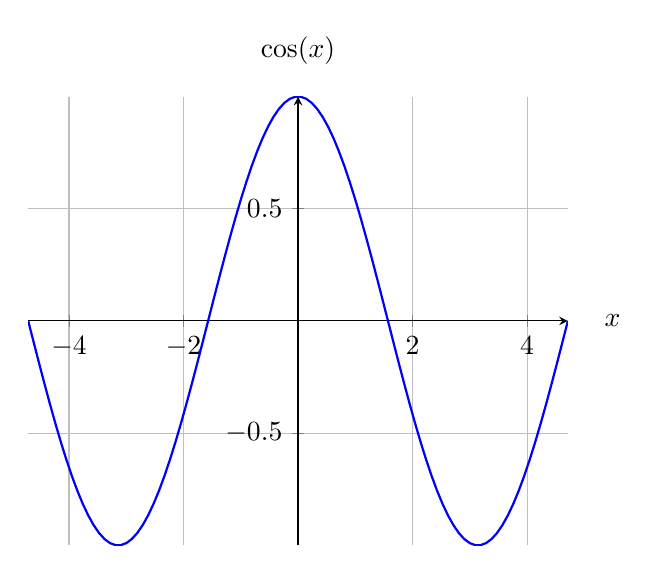
\begin{tikzpicture}
		\begin{axis}[
			xlabel=$x$,
			ylabel=$\cos(x)$,
			domain=-3/2*pi:3/2*pi,
			samples=100,
			axis lines=middle,
			grid=both,
			every axis y label/.style={at={(ticklabel* cs:1.05)}, anchor=south},
			every axis x label/.style={at={(ticklabel* cs:1.05)}, anchor=west},
			]
			\addplot[blue, thick] {cos(deg(x))};
		\end{axis}
	\end{tikzpicture}
	\caption{Cosine function.}
	\label{cos}
\end{figure}

Now we will take a step back and try to achieve the mysterious number for the approximation ratio. Let $\theta_{ij}$ be the angle between $v_{i}$ and $v_{j}$. Then for $\{i,j\} \in E$, its contribution to the objective (in VP) is $\frac{1 - \cos \theta_{ij}}{2}$.

\begin{lemma}[no proof]
	For each $x \in \langle 0, \pi \rangle$ and $\alpha = 0,87856$ it holds that
	
	$$
	\frac{x}{\pi} \geq \alpha \frac{1 - \cos x}{2}
	$$
\end{lemma}

The meaning of it is shown on the picture \ref{meaning}.

\begin{figure}[!ht]\centering
	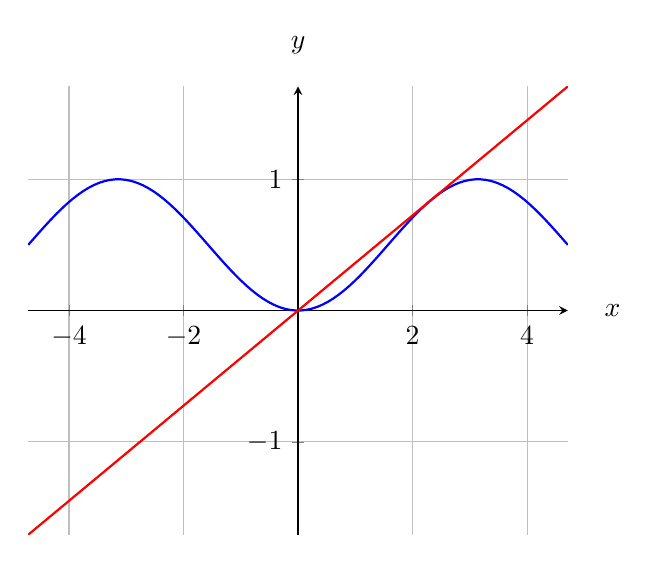
\begin{tikzpicture}
		\begin{axis}[
			xlabel=$x$,
			ylabel=$y$,
			domain=-3/2*pi:3/2*pi,
			samples=100,
			axis lines=middle,
			grid=both,
			every axis y label/.style={at={(ticklabel* cs:1.05)}, anchor=south},
			every axis x label/.style={at={(ticklabel* cs:1.05)}, anchor=west},
			legend pos=outer north east,
			]
			\addplot[blue, thick, label=($(1 - \cos(x)) /2$)] {(1 - cos(deg(x))) / 2};
			\addplot[red, thick, label=($x/(\pi \cdot \alpha)$)] {x / (0.87856 * pi)};
			\legend{}
		\end{axis}
	\end{tikzpicture}
	\caption{The \textcolor{red}{red} function is for $x/(\pi \cdot \alpha)$ and \textcolor{blue}{blue} for $(1 - \cos(x)) /2$.}
	\label{meaning}
\end{figure}

\begin{lemma}
	For $\{i,j\} \in E$ $\Pr [i \text{ and } j \text{ are separated}] = \frac{\theta_{ij}}{\pi}$.
\end{lemma}

\begin{proof}
	Consider the projection of $r$ to the plane defined by $v_i$, $v_j$. Let $W$ be the objective value of our solution:
	
	$$
	\begin{aligned}
		\E [W] & =    & \sum_{\{i,j\} \in E} \frac{\theta_{ij}}{\pi} & \quad \text{(by linearity of expectation)} \\
		       & \geq & \alpha \sum_{\{i,j\} \in E} \frac{1 - \cos (\theta_{ij})}{2} & \quad \text{(by the first lemma)} \\
		       & =    & \alpha \sum_{\{i,j\} \in E} \frac{1 - v_{i}^T v_{j}}{2} & \quad \textbf{(this is our objective functions of VP)} \\
		       & \geq & \alpha \cdot OPT & \quad \text{(because VP is a relaxation)}
	\end{aligned}
	$$
\end{proof}
	\chapter{Edge disjoint path problem}

Some readers may already know what is edge disjoint path problem and also some basic algorithms. But we will have a brief introduction to this topic.

\begin{itemize}
	\item \textbf{INPUT}: $G=(V,E)$ and $(s_{i}, t_{i}) \in V^2$ for all $i \in [k]$.
	\item \textbf{OUTPUT}: $I \subseteq [k]$ and an $s_{i}-t_{i}$ path $P_{i}$ for each $i \in I$, s.t. the selected paths are edge disjoint.
	\item \textbf{OBJECTIVE}: $\max |I|$.
\end{itemize}

It is known that this particular problem is NP-hard. So we will again show some approximation to this problem. \textit{Note: for any fix $k$ it is solvable in polynomial time on undirected graph. But for directed graphs it is NP-hard for $k = 2$.} We will introduce an greedy algorithm that has an parameter.

\begin{algorithm}
	\caption{Greedy algorithm with a catch for parameter $\sqrt{m}$}
	\begin{algorithmic}[1]
		\State $I = \emptyset$
		\While{$\exists i \notin I$ and $\exists s_{i}-t_{i}$ path in $G$, s.t. $|P_{i}| \leq \sqrt{m}$}
			\State $I = I \cup \{i\}$, keep $P_{i}$, $G = G \setminus P_{i}$
		\EndWhile
	\end{algorithmic}
\end{algorithm}

We will denote $OPT$ as the optimal solution of the problem. It will be either a set of paths or set of indexes. Then we will denote $OPT_{S} = \{P \in OPT \mid |P| \leq \sqrt{m}\}$, where the length of a path is set as the number of edges. Then $OPT_{L} = OPT \setminus OPT_{S}$ and $ALG$ as the set given by the algorithm.

Now take the set $OPT_{S} \setminus ALG$. That is path between $s_{i}$ and $t_{i}$ is in this set if there exists $s_{j}-t_{j}$ path obtained by the algorithm which shares an edge. This path has length at most $\sqrt{m}$ and there are $|ALG|$ paths. Thus altogether $|OPT_{S} \setminus ALG| \leq \sqrt{m} |ALG|$.

Next we may see that $|OPT_{L}| \leq \sqrt{m}$, because we have $m$ edges and each one of them is at least $\sqrt{m}$ long. Now we may conclude altogether following result.

$$
|OPT| \leq |OPT_{L}| + |OPT_{S} \setminus ALG| + |ALG| \leq O(\sqrt{m}) |ALG|
$$

Now one can see where the catch in the algorithm is. Consider that there are no such short paths. The algorithm will output no path at all. To fix this we need to change the algorithm such that it will always output at least one path. If there is none then $OPT$ is 0 as well.

\begin{algorithm}
	\caption{Greedy ($\sqrt{m}$)}
	\begin{algorithmic}[1]
		\State $I = \emptyset$
		\While{$\exists i \notin I$ and $\exists s_{i}-t_{i}$ path in $G$, s.t. $|P_{i}| \leq \sqrt{m}$}
		\State $I = I \cup \{i\}$, keep $P_{i}$, $G = G \setminus P_{i}$
		\EndWhile
		\If{\textcolor{purple}{$I = \emptyset$}}
			\State \textcolor{purple}{Connect any $s_{i}-t_{i}$ path if possible.}
		\EndIf
	\end{algorithmic}
\end{algorithm}

Thus we have shown an algorithm that is a $\sqrt{m}$-approximation. Now we consider running the same algorithm but we change the parameter from $\sqrt{m}$ to $n^{2/3}$. Can we obtain $n^{2/3}$-approximation?

\begin{thm}[Khana, Chedari]
	Given an instance of the sum multi-commodity flow problem $G =(V,E), (s_{i}, t_{i}) \in V^2$ for all $i \in [k]$ such that $(\forall i) d(s_{i}, t_{i}) \leq l$, then the max multi-commodity flow is $O(\frac{n^2}{l^2})$.
\end{thm}

Before proving this we will show the consequences for our problem. Lets use the algorithm Greedy$(n^{2/3})$. Assume there $\exists P_{i} \in ALG, |P_{i}| \leq n^{2/3}$. Otherwise we use the theorem on the network obtained by $G$ and setting all capacities to one. Then all edges are at least $n^{2/3}$ length so we get the max multi-commodity flow is $O(\frac{n^{2}}{n^{4/3}}) = O(n^{2/3})$. Therefore it means if we choose just one path the approximation ratio will still be $O(n^{2/3})$.

Denote $OPT_{easy} = \{P \in OPT \mid \exists Q \in ALG : Q \cap P \neq \emptyset\}$. With this we know that $|OPT_{easy}| \leq n^{2/3} |ALG|$ by the same argument as it was already mentioned before.

We will look at $\forall (s_{i}, t_{i}) \in (OPT \setminus OPT_{easy}) \setminus ALG$. What can we say about such $d(s_{i}, t_{i})$ at the end of the loop of the algorithm. Clearly because it was not chosen either there is some intersection with another path, but this is remove by $OPT_{easy}$, so the other option is only that $d(s_{i}, t_{i}) > n^{2/3}$. Hence $|(OPT \setminus OPT_{easy}) \setminus ALG| \leq O(n^{2/3})$ by the theorem and the same argument which was already mentioned. Altogether we have:

$$
|OPT| \leq |OPT_{easy}| + |(OPT \setminus OPT_{easy}) \setminus ALG| + |ALG| = O(n^{2/3}) |ALG|
$$

Now we only need to proof the theorem since it is the base of our arguments for obtaining $O(n^{2/3})$-approximation algorithm.

\begin{proof}
	We will split the vertices into two sets:
	
	\begin{enumerate}
		\item \textbf{low degree vertex} are when $\deg(v) \leq \frac{6 n}{l}$
		\item \textbf{high degree vertex} are when $\deg(v) > \frac{6 n}{l}$
	\end{enumerate}
	
	Also we will assume $l$ is a multiple of 6. Otherwise it get lost in the $O$ notation. To finish the proof we will use an observation.
	
	\begin{observ}
		Any $s_{i}-t_{i}$ path (denote it as $s-t$) uses at least $l/6$ low degree vertices.
	\end{observ}
	
	\begin{proof}[Proof of observation]
		Consider running BFS on the graph starting from $s$. We denote $L_{i} = \{u \in V : d(s,u) = i\}$. Note that edges are only within one layer or only between adjacent layers. Let $B_{i}$ be a block of three consecutive layers $\{L_{3i}, L_{3i+1}, L_{3i+2}\}$. Because the length to $t$ is at least $l$ then there is at least $l/3$ blocks. Assume that $< l/6$ layers consists of only low degree vertices. Otherwise the observation obviously holds. Now discard all blocks containing a layer of only low degree vertices. As there are $\geq l/3$ blocks at least $\geq l/6$ blocks remain. Then the smallest remaining block is of size $\leq \frac{n}{l/6} = 6n/l$ which can be seen by pigeonhole principle. For the vertices in the middle layer we know all neighbors are within the block. Therefore it is a low degree vertex. This is a contradiction because we still have a block having one layer with low degree vertices only.
	\end{proof}
	
	Now for the theorem we know a \textbf{unit} of flow between any pair $s_{i}-t_{i}$ consumes $\mathbf{\Omega(l)}$ cpacity of edges adjacent to low degree vertices. And the total capacity adjacent to low degree vertices is $\leq n \deg(v) \leq n (6n/l) = O(n^2/l)$. Which gives us $O(n^2/l^2)$.
\end{proof}

This is an example of greedy algorithm and the fact that using it with different parameter may result in better approximation, but the analysis is way harder. We also saw using flows to limit paths, but this has also its limits. We will show a counterexample a graph called \textbf{Brick wall}.

\begin{figure}[!ht]\centering
	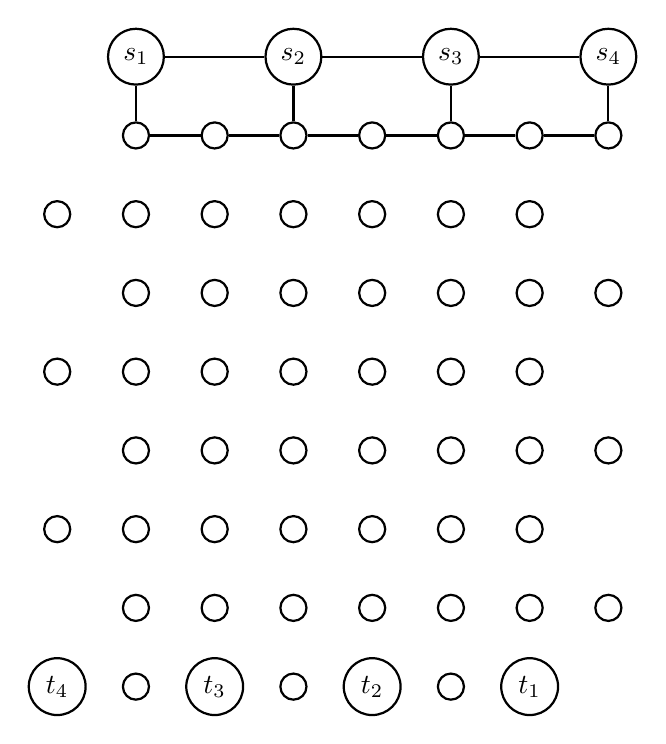
\begin{tikzpicture}[node distance={10mm}, thick, main/.style = {draw, circle}]
		\node[main] (1) {$s_{1}$};
		\node[main] (5) [below of=1] {};
		\node[main] (6) [right of=5] {};
		\node[main] (7) [right of=6] {};
		\node[main] (2) [above of=7] {$s_{2}$};
		
		\node[main] (8) [right of=7] {};
		\node[main] (9) [right of=8] {};
		\node[main] (3) [above of=9] {$s_{3}$};
		
		\node[main] (10) [right of=9] {};
		\node[main] (11) [right of=10] {};
		\node[main] (4) [above of=11] {$s_{4}$};
		
		\node[main] (13) [below of=5] {};
		\node[main] (12) [left of=13] {};
		\node[main] (14) [right of=13] {};
		\node[main] (15) [right of=14] {};
		\node[main] (16) [right of=15] {};
		\node[main] (17) [right of=16] {};
		\node[main] (18) [right of=17] {};
		
		\node[main] (22) [below of=13] {};
		\node[main] (23) [right of=22] {};
		\node[main] (24) [right of=23] {};
		\node[main] (25) [right of=24] {};
		\node[main] (26) [right of=25] {};
		\node[main] (27) [right of=26] {};
		\node[main] (28) [right of=27] {};
		
		\node[main] (33) [below of=22] {};
		\node[main] (32) [left of=33] {};
		\node[main] (34) [right of=33] {};
		\node[main] (35) [right of=34] {};
		\node[main] (36) [right of=35] {};
		\node[main] (37) [right of=36] {};
		\node[main] (38) [right of=37] {};
		
		\node[main] (42) [below of=33] {};
		\node[main] (43) [right of=42] {};
		\node[main] (44) [right of=43] {};
		\node[main] (45) [right of=44] {};
		\node[main] (46) [right of=45] {};
		\node[main] (47) [right of=46] {};
		\node[main] (48) [right of=47] {};
		
		\node[main] (53) [below of=42] {};
		\node[main] (52) [left of=53] {};
		\node[main] (54) [right of=53] {};
		\node[main] (55) [right of=54] {};
		\node[main] (56) [right of=55] {};
		\node[main] (57) [right of=56] {};
		\node[main] (58) [right of=57] {};
		
		\node[main] (62) [below of=53] {};
		\node[main] (63) [right of=62] {};
		\node[main] (64) [right of=63] {};
		\node[main] (65) [right of=64] {};
		\node[main] (66) [right of=65] {};
		\node[main] (67) [right of=66] {};
		\node[main] (68) [right of=67] {};
		
		\node[main] (73) [below of=62] {};
		\node[main] (72) [left of=73] {$t_{4}$};
		\node[main] (74) [right of=73] {$t_{3}$};
		\node[main] (75) [right of=74] {};
		\node[main] (76) [right of=75] {$t_{2}$};
		\node[main] (77) [right of=76] {};
		\node[main] (78) [right of=77] {$t_{1}$};
		%12 13 14 15 16 17 18
		%22 23 24 25 26 27 28
		
		\draw (1) -- (2);
		\draw (2) -- (3);
		\draw (3) -- (4);
		
		\draw (1) -- (5);
		\draw (2) -- (7);
		\draw (3) -- (9);
		\draw (4) -- (11);
		
		\draw (5) -- (6);
		\draw (6) -- (7);
		\draw (7) -- (8);
		\draw (8) -- (9);
		\draw (9) -- (10);
		\draw (10) -- (11);
	\end{tikzpicture}
	\caption{Example of a \textbf{brick wall} graph for $k = 4$.}
	\label{brick-wall}
\end{figure}

The graph you may see at the picture \ref{brick-wall} is planar. Also it can be generalized to $k$ where there are $k$ pairs of bricks underneath. The edge disjoint problem optimum is 1, which we can see on picture \ref{edg}. And the max multi flow optimum is at least $k/2 = O(\sqrt{n})$, which can be seen on picture \ref{max-flow}.


\begin{figure}[!ht]\centering
	\caption{Edge disjoint problem.}
	\label{edg}
\end{figure}

\begin{figure}[!ht]\centering
	\caption{Max multi flow optimum.}
	\label{max-flow}
\end{figure}
\end{document}

